\section{Introduction}
\label{sec:dof-intro}

OpenDTrace programs are persistently encoded in the DOF format so that
they may be embedded in other programs (for example, in an ELF file)
or in the DTrace driver configuration file for use in anonymous
tracing.  The DOF format is versioned and extensible so that it can be
revised and so that internal data structures can be modified or
extended compatibly.  All DOF structures use fixed-size types, so the
32-bit and 64-bit representations are identical and consumers can use
either data model transparently.

\subsection{Stable Storage Format}
\label{sec:dof-stable-storage}

\begin{figure}[h]
  \centering
  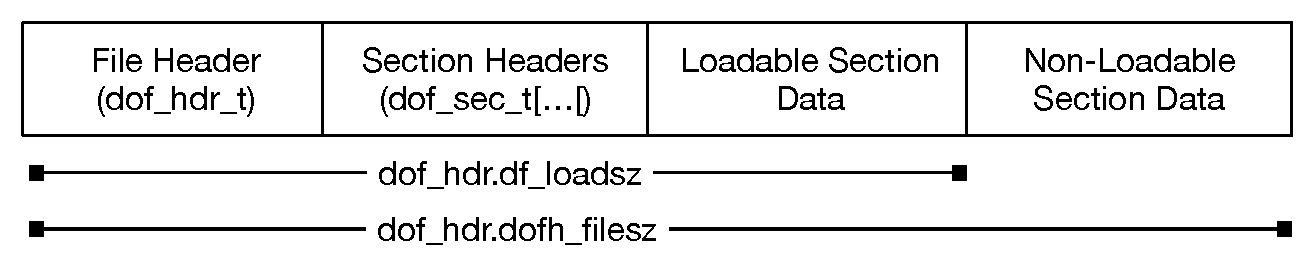
\includegraphics[width=.8\textwidth]{dof-stable-format}
  \caption{Stable Storage Format}
  \label{fig:dof-stable-storage-format}
\end{figure}

When a DOF file resides on stable storage it is stored in the format
shown in Figure~\ref{fig:dof-stable-storage-format}. The file header
stores meta-data including a magic number, data model for the
instrumentation, data encoding, and properties of the DIF code within.
The header describes its own size and the size of the section headers.
By convention, an array of section headers follows the file header,
and then the data for all loadable sections and sections which cannot
be loaded, also called unloadable sections.  This data layout permits
consumer code to easily download the headers and all loadable data
into the DTrace driver in one contiguous chunk, omitting other
extraneous sections.

The section headers describe the size, offset, alignment, and section
type for each section.  Sections are described using a set of \verb|#defines|
that tell the consumer what kind of data is expected.  Sections can
contain links to other sections by storing a \verb|dof_secidx_t|, an index
into the section header array, inside of the section data structures.
The section header includes an entry size so that sections with data
arrays can grow their structures.

The DOF data itself can contain many snippets of DIF (i.e. more than
one DIF object or DIFO), which are represented themselves as a
collection of related DOF sections.  This permits us to change the set
of sections associated with a DIFO over time, and also permits us to
encode DIFOs that contain different sets of sections.  When a DOF
section wants to refer to a DIFO, it stores the \verb|dof_secidx_t| of
a section of type \verb|DOF_SECT_DIFOHDR|.  This section's data is
then an array of \verb|dof_secidx_t|'s which in turn denote the
sections associated with this DIFO.

This loose coupling of the file structure (header and sections) to the
structure of the DTrace program itself (enebled code block
descriptions, action descriptions, and DIFOs) permits activities such
as relocation processing to occur in a single pass without having to
understand D program structure.

Finally, strings are always stored in ELF-style string tables along
with a string table section index and string table offset.  Therefore
strings in DOF are always arbitrary-length and not bound to the
current implementation.

\begin{table}
  \centering
\begin{tabular}{|l|l|l|}
\hline
  Name & Loadable & Comment\\
\hline
\verb|DOF_SECT_NONE| & N & null section\\
\verb|DOF_SECT_COMMENTS| & N & compiler comments\\
\verb|DOF_SECT_SOURCE| & N & D program source code\\
\verb|DOF_SECT_ECBDESC| & Y & \verb|dof_ecbdesc_t|\\
\verb|DOF_SECT_PROBEDESC| & Y & \verb|dof_probedesc_t|\\
\verb|DOF_SECT_ACTDESC| & Y & \verb|dof_actdesc_t| array\\
\verb|DOF_SECT_DIFOHDR| & Y & \verb|dof_difohdr_t| (variable length)\\
\verb|DOF_SECT_DIF| & Y & \verb|uint32_t array| of byte code\\
\verb|DOF_SECT_STRTAB| & Y & string table\\
\verb|DOF_SECT_VARTAB| & Y & \verb|dtrace_difv_t| array\\
\verb|DOF_SECT_RELTAB| & Y & \verb|dof_relodesc_t| array\\
\verb|DOF_SECT_TYPTAB| & Y & \verb|dtrace_diftype_t| array\\
\verb|DOF_SECT_URELHDR| & Y & \verb|dof_relohdr_t| (user relocations)\\
\verb|DOF_SECT_KRELHDR| & Y & \verb|dof_relohdr_t| (kernel relocations)\\
\verb|DOF_SECT_OPTDESC| & Y & \verb|dof_optdesc_t| array\\
\verb|DOF_SECT_PROVIDER| & Y & \verb|dof_provider_t|\\
\verb|DOF_SECT_PROBES| & Y & \verb|dof_probe_t| array\\
\verb|DOF_SECT_PRARGS| & Y & \verb|uint8_t array| (probe arg mappings)\\
\verb|DOF_SECT_PROFFS| & Y & \verb|uint32_t array| (probe arg offsets)\\
\verb|DOF_SECT_INTTAB| & Y & \verb|uint64_t array|\\
\verb|DOF_SECT_UTSNAME| &  & struct utsname\\
\verb|DOF_SECT_XLTAB| & Y & \verb|dof_xlref_t| array\\
\verb|DOF_SECT_XLMEMBERS| & Y & \verb|dof_xlmember_t| array\\
\verb|DOF_SECT_XLIMPORT| & Y & \verb|dof_xlator_t|\\
\verb|DOF_SECT_XLEXPORT| & Y & \verb|dof_xlator_t|\\
\verb|DOF_SECT_PREXPORT| & Y & \verb|dof_secidx_t| array (exported objs)\\
\verb|DOF_SECT_PRENOFFS| & Y & \verb|uint32_t array| (enabled offsets)\\
\hline
\end{tabular}
  \caption{DOF Section Descriptions}
  \label{tab:dof-sections}
\end{table}


%%% Local Variables:
%%% mode: latex
%%% TeX-master: "dtrace-specification"
%%% End:
